\documentclass[a4paper, 11pt]{article}
\usepackage[a4paper, text={17cm, 24cm}, left={2cm}, top={3cm}]{geometry}
\usepackage[utf8]{inputenc}
\usepackage{times}
\usepackage[czech]{babel}
\usepackage{multirow}
\usepackage{graphics}
\usepackage[ruled, noline, czech, linesnumbered, longend]{algorithm2e}
\usepackage{setspace}
\usepackage{pict2e}
\usepackage[unicode]{hyperref}
\usepackage{caption}

\renewcommand{\uv}[1]{\quotedblbase #1\textquotedblleft}
\urlstyle{same}

\date{}

\begin{document}
%%
%%  TITULNI STRANA
%%
\begin{titlepage}

\begin{center}
\LARGE
\textsc{\Huge Vysoké učení technické v Brně}\\
\textsc{\huge Fakulta informačních technologií}\\
\vspace{\stretch{0.382}}
Typografie a publikování\,--\,3. projekt\\[0.4em]
{\Huge Tabulky a obrázky}
\vspace{\stretch{0.618}}
\end{center}
{\Large \today \hfill Dominik Horký (xhorky32)}

\end{titlepage}

%%
%%  UVODNI STRANA
%%  (1, 2, 2.1, 2.2)
%%

% 1
\section{Úvodní strana}
Název práce umístěte do zlatáho řezu a nezapomeňte uvést dnešní datum a vaše jméno a příjmení.

% 2
\section{Tabulky}
Pro sázení tabulek můžeme použít buď prostředí\verb| tabbing |nebo prostředí\verb| tabular|.

% 2.1
\subsection{Prostředí\texttt{ tabbing }}
Při použití\verb| tabbing |vypadá tabulka následovně:
\begin{tabbing}
aaaaaaaaaaaaaaaa \= 0000,00 \= 0000 kg \kill
\textbf{Ovoce} \> \textbf{Cena} \> \textbf{Množství} \\
Jablka \> 25,90 \> 3 kg \\
Hrušky \> 27,40 \> 2,5 kg \\
Vodní melouny \> 35,-- \> 1 kus \\
\end{tabbing}
\noindent
Toto prostředí se dá také použít pro sázení algoritmů, ovšem vhodnější je použít 
prostředí\verb| algorithm |nebo \verb|algorithm2e |(viz sekce \ref{section:3}).

% 2.2
\subsection{Prostředí\texttt{ tabular }}
\catcode`\-=12

Další možností, jak vytvořit tabulku, je použít prostředí\verb| tabular|. Tabulky pak 
budou vypadat takto\footnote{Kdyby byl problem s \texttt{ cline,} zkuste se podívat třeba sem: 
\url{http://www.abclinuxu.cz/tex/poradna/show/325037}.}:
\bigskip
% TABULKA 1 
% (kurzy měn)
%
\begin{table}[h]
\centering
\begin{tabular}{|l|c|c|}
\hline
    & \multicolumn{2}{c|}{\textbf{Cena}} \\
    \cline{2-3}
    \textbf{Měna} & \textbf{nákup} & \textbf{prodej} \\ \hline
    EUR & 25,475 & 27,045 \\
    GBP & 28,835 & 30,705 \\
    USD & 22,943 & 24,357 \\
\hline
\end{tabular} \caption{Tabulka kurzů k dnešnímu dni} \label{tab:1}
\end{table}
\bigskip
% TABULKA 2 
% (čtyřhodnotová logika)
%
\begin{table}[h]
\centering
\begin{tabular}{|c|c|}
\hline
    $A$ & $\neg A$  \\ \hline
    \textbf{P} & N \\ \hline
    \textbf{O} & O \\ \hline
    \textbf{X} & X \\ \hline
    \textbf{N} & P \\
\hline
\end{tabular}
\begin{tabular}{|c|c|c|c|c|c|}
\hline
    \multicolumn{2}{|c|}{\multirow{2}{*}{$A \land B$}} & \multicolumn{4}{c|}{$B$} \\
    \cline{3-6}
    \multicolumn{2}{|c|}{} & \textbf{P} & \textbf{O} & \textbf{X} & \textbf{N} \\
    \cline{1-6}
    \multirow{4}{*}{$A$} & \textbf{P} & P & O & X & N \\
    \cline{2-6}
    & \textbf{O} & O & O & N & N \\
    \cline{2-6}
    & \textbf{X} & X & N & X & N \\
    \cline{2-6}
    & \textbf{N} & N & N & N & N \\
\hline
\end{tabular}
\begin{tabular}{|c|c|c|c|c|c|}
\hline
    \multicolumn{2}{|c|}{\multirow{2}{*}{$A \lor B$}} & \multicolumn{4}{c|}{$B$} \\
    \cline{3-6}
    \multicolumn{2}{|c|}{} & \textbf{P} & \textbf{O} & \textbf{X} & \textbf{N} \\
    \cline{1-6}
    \multirow{4}{*}{$A$} & \textbf{P} & P & P & P & P \\
    \cline{2-6}
    & \textbf{O} & P & O & P & O \\
    \cline{2-6}
    & \textbf{X} & P & P & X & X \\
    \cline{2-6}
    & \textbf{N} & P & O & X & N \\
\hline
\end{tabular}
\begin{tabular}{|c|c|c|c|c|c|}
\hline
    \multicolumn{2}{|c|}{\multirow{2}{*}{$A \rightarrow B$}} & \multicolumn{4}{c|}{$B$} \\
    \cline{3-6}
    \multicolumn{2}{|c|}{} & \textbf{P} & \textbf{O} & \textbf{X} & \textbf{N} \\
    \cline{1-6}
    \multirow{4}{*}{$A$} & \textbf{P} & P & O & X & N \\
    \cline{2-6}
    & \textbf{O} & P & O & P & O \\
    \cline{2-6}
    & \textbf{X} & P & P & X & X \\
    \cline{2-6}
    & \textbf{N} & P & P & P & P \\
\hline
\end{tabular} \caption{Protože Kleeneho trojhodnotová logika už je \uv{zastaralá}, uvádíme si zde příklad čtyřhodnotové logiky} \label{tab:2}
\end{table}
\bigskip
\pagebreak

\newpage
%%
%%  ALGORITMY A OBRAZKY
%%  (3, 4)
%%

% 3
\section{Algoritmy} \label{section:3}
\setlength{\parskip}{0em}
Pokud budeme chtít vysázet algoritmus, můžeme použít 
prostředí\verb| algorithm|\footnote{Pro nápovědu, jak zacházet s
prostředím\texttt{ algorithm,} můžeme zkusit tuhle stránku:\\
\url{http://ftp.cstug.cz/pub/tex/CTAN/macros/latex/contrib/algorithms/algorithms.pdf}.} \ nebo\verb| algorithm2e|\footnote{Pro\texttt{ algorithm2e }zase tuhle:
\url{http://ftp.cstug.cz/pub/tex/CTAN/macros/latex/contrib/algorithm2e/doc/algorithm2e.pdf}.}.
Příklad použití prostředí\verb| algorithm2e |viz Algoritmus \ref{alg:1}.
\bigskip

% algoritmus
\IncMargin{1.5em}
\begin{algorithm} 
\setstretch{0.92}
\SetNlSty{}{}{:}

\SetAlgoNlRelativeSize{-1}
\SetInd{0em}{1em}
\Indm \Indmm

\KwIn{ ($X_{t-1}, u_t, z_t$)}
\KwOut{ $X_t$}

\Indp \Indpp
\SetInd{1em}{1em}
\BlankLine

$\overline{X_t} = X_t = 0$\\
\For{$k = 1$ \emph{to} $M$}{
$x_t^{[k]} =$ \emph{sample\_motion\_model}$ (u_t,x_{t-1}^{[k]})$\\
$\omega_t^{[k]} =$ \emph{measurement\_model}$(z_t,x_t^{[k]},m_{t-1})$\\
$m_t^{[k]} = updated\_occupancy\_grid(z_t,x_t^{[k]},m_{t-1}^{[k]})$\\
$\overline{X_t} = \overline{X_t} + \langle x_x^{[m]}, \omega_t^{[m]} \rangle$\\
}
\For{$k = 1$ \emph{to} $M$}{
draw $i$ with probability $\approx \omega_t^{[i]}$\\
add $\langle x_x^{[k]},m_t^{[k]} \rangle$ to $X_t$\\
}
\Return{ $X_t$}
\caption{\textsc{Fast}SLAM} \label{alg:1}

\end{algorithm}

% 4
\section{Obrázky}

Do našich článků můžeme samozřejmě vkládat obrázky. Pokud je obrázkem fotografie,
můžeme klidně použít bitmapový soubor. Pokud by to ale mělo být nějaké schéma nebo
něco podobného, je dobrým zvykem takovýto obrázek vytvořit vektorově.
\setlength{\parskip}{0.1em}
\begin{figure}[h]
\centering
\scalebox{0.4}{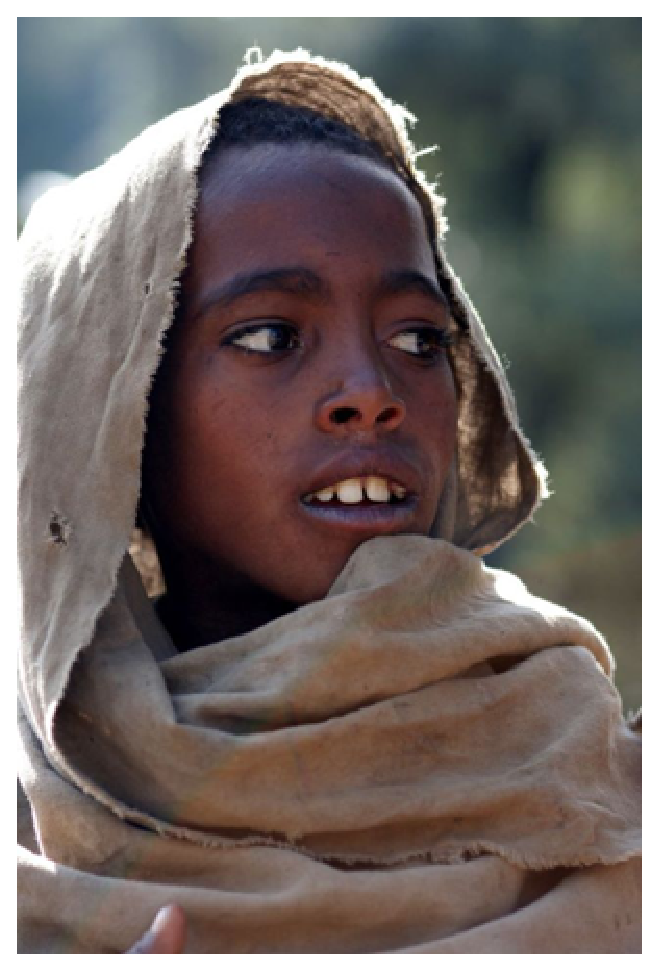
\includegraphics{data/etiopan.eps}}\hspace{0.24mm}\reflectbox{\scalebox{0.4}{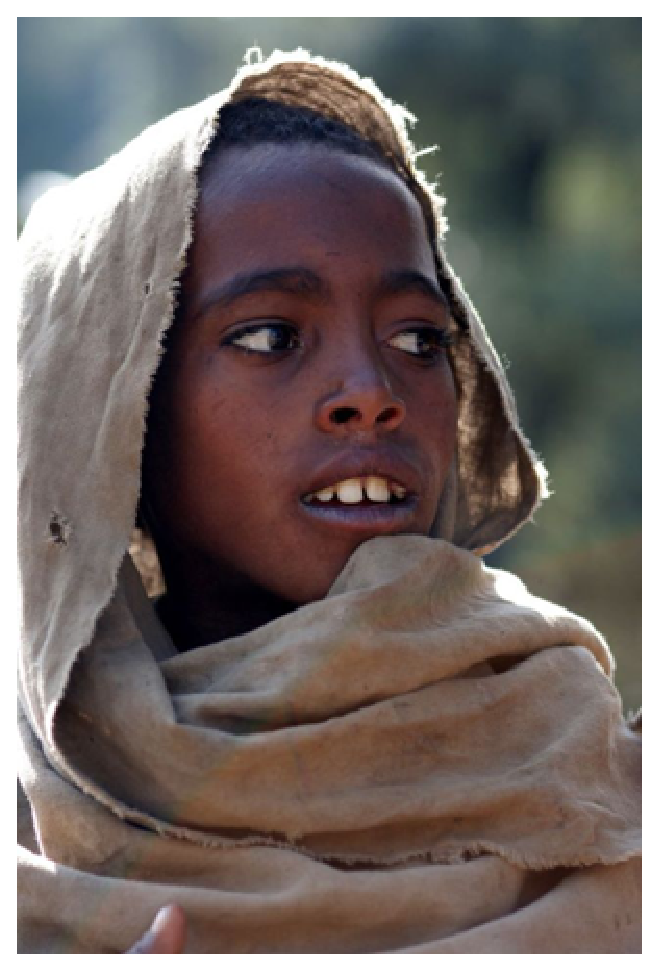
\includegraphics{data/etiopan.eps}}}
\medskip
\caption{Malý Etiopánek a jeho bratříček} \label{pic:1}
\medskip
\end{figure}

\newpage
%%
%%  ROZDILY MEZI TYPY OBRAZKU
%%  (vektor vs bitmap)
%%
Rozdíl mezi vektorovým \dots 

\begin{figure}[h]
\centering
\scalebox{0.4}{
\includegraphics{data/oniisan.eps}} 
\medskip
\caption{Vektorový obrázek} \label{pic:2}
\end{figure}
\setlength{\parskip}{1em}
\noindent\dots\ a bitmapovým obrázkem
\begin{figure}[h]
\centering
\scalebox{0.6}{
\includegraphics{data/oniisan2.eps}} 
\medskip
\caption{Bitmapový obrázek} \label{pic:3}
\end{figure} 

\noindent se projeví například při zvětšení.\par\setlength{\parskip}{0em}
Odkazy (nejen ty) na obrázky \ref{pic:1}, \ref{pic:2} a \ref{pic:3}, na tabulky \ref{tab:1} a \ref{tab:2} a také na algoritmus \ref{alg:1} jsou udělány pomocí křížových odkazů. Pak je ovšem potřeba zdrojový soubor přeložit dvakrát.\par
Vektorové obrázky lze vytvořit i přímo v \LaTeX u, například pomocí prostředí\verb| picture|.

\newpage
%%
%%  VLASTNI TVORBA - OBRAZEK BUDOVY
%%  (moderni budova 21. st.)
%%

\begin{figure}
\setlength{\unitlength}{0.8cm}
\begin{picture}(20,25)

\thicklines
%% budova
% hlavni linie budovy
\put(2,0){\line(18,0){16}}
\put(2,0){\line(0,18){18}}
\put(2,18){\line(16,0){16}}
\put(18,0){\line(0,18){18}}
% 3D efekt
\put(0,2){\line(0,18){18}}
\put(2,0){\line(-2,2){2}}
\put(2,18){\line(-2,2){2}}
\put(0.3,20){\line(18,0){1.7}}
\put(5,20){\line(18,0){11}}
\put(17.7,18.3){\line(-2,2){1.7}}
% 'zabradli' strechy
\put(2,18.3){\line(16,0){16}}
\put(2,18){\line(0,0.3){0.3}}
\put(2,18.3){\line(-2,2){2}}
\put(0,20){\line(0,0.3){0.3}}
\put(0,20.3){\line(2,0){2}}
\put(5,20.3){\line(11,0){11}}
\put(16,20.3){\line(2,-2){2}}
\put(16,20.3){\line(0,-0.3){0.3}}
\put(18,18){\line(0,0.3){0.3}}

% vchod
\put(8,0){\line(0,2){2.3}} % hlavni linie
\put(10,0){\line(0,2){2.3}}
\put(8,2.3){\line(2,0){2}}
\put(12,0){\line(0,2){2.3}}
\put(10,2.3){\line(2,0){2}}

\put(7.8,0){\line(0,2){2.5}} % vnejsi okraje vchodu
\put(12.2,0){\line(0,2){2.5}}
\put(7.8,2.5){\line(4.4,0){4.4}}

\put(9.85,0){\line(0,1){2.3}} % vnitrni okraje dveri
\put(10.15,0){\line(0,1){2.3}}

\put(10,2.35){\circle*{0.15}} % detail - senzor (otevirani dveri)
% okna
\put(3,2.2){\line(3,0){3}} %1x1
\put(3,2.3){\line(3,0){3}}
\put(3,4.3){\line(3,0){3}}
\put(3,4.4){\line(3,0){3}}
\put(3,2.3){\line(0,2){2}}
\put(6,2.3){\line(0,2){2}}
\put(3,3.3){\line(3,0){3}}
\put(4.5,2.3){\line(0,2){2}}

\put(3,5.2){\line(3,0){3}} %1x2
\put(3,5.3){\line(3,0){3}}
\put(3,7.3){\line(3,0){3}}
\put(3,7.4){\line(3,0){3}}
\put(3,5.3){\line(0,2){2}}
\put(6,5.3){\line(0,2){2}}
\put(3,6.3){\line(3,0){3}}
\put(4.5,5.3){\line(0,2){2}}

\put(3,8.2){\line(3,0){3}} %1x3
\put(3,8.3){\line(3,0){3}}
\put(3,10.3){\line(3,0){3}}
\put(3,10.4){\line(3,0){3}}
\put(3,8.3){\line(0,2){2}}
\put(6,8.3){\line(0,2){2}}
\put(3,9.3){\line(3,0){3}}
\put(4.5,8.3){\line(0,2){2}}

\put(3,11.2){\line(3,0){3}} %1x4
\put(3,11.3){\line(3,0){3}}
\put(3,13.3){\line(3,0){3}}
\put(3,13.4){\line(3,0){3}}
\put(3,11.3){\line(0,2){2}}
\put(6,11.3){\line(0,2){2}}
\put(3,12.3){\line(3,0){3}}
\put(4.5,11.3){\line(0,2){2}}

\put(3,14.2){\line(3,0){3}} %1x5
\put(3,14.3){\line(3,0){3}}
\put(3,16.3){\line(3,0){3}}
\put(3,16.4){\line(3,0){3}}
\put(3,16.43){\line(3,0){3}}
\put(3,14.3){\line(0,2){2}}
\put(6,14.3){\line(0,2){2}}
\put(3,15.3){\line(3,0){3}}
\put(4.5,14.3){\line(0,2){2}}

\put(17,2.2){\line(-3,0){3}} %3x1
\put(17,2.3){\line(-3,0){3}}
\put(17,4.3){\line(-3,0){3}}
\put(17,4.4){\line(-3,0){3}}
\put(17,2.3){\line(0,2){2}}
\put(14,2.3){\line(0,2){2}}
\put(17,3.3){\line(-3,0){3}}
\put(15.5,2.3){\line(0,2){2}}

\put(17,5.2){\line(-3,0){3}} %3x2
\put(17,5.3){\line(-3,0){3}}
\put(17,7.3){\line(-3,0){3}}
\put(17,7.4){\line(-3,0){3}}
\put(17,5.3){\line(0,2){2}}
\put(14,5.3){\line(0,2){2}}
\put(17,6.3){\line(-3,0){3}}
\put(15.5,5.3){\line(0,2){2}}

\put(17,8.2){\line(-3,0){3}} %3x3
\put(17,8.3){\line(-3,0){3}}
\put(17,10.3){\line(-3,0){3}}
\put(17,10.4){\line(-3,0){3}}
\put(17,8.3){\line(0,2){2}}
\put(14,8.3){\line(0,2){2}}
\put(17,9.3){\line(-3,0){3}}
\put(15.5,8.3){\line(0,2){2}}

\put(17,11.2){\line(-3,0){3}} %3x4
\put(17,11.3){\line(-3,0){3}}
\put(17,13.3){\line(-3,0){3}}
\put(17,13.4){\line(-3,0){3}}
\put(17,11.3){\line(0,2){2}}
\put(14,11.3){\line(0,2){2}}
\put(17,12.3){\line(-3,0){3}}
\put(15.5,11.3){\line(0,2){2}}

\put(17,14.2){\line(-3,0){3}} %3x5
\put(17,14.3){\line(-3,0){3}}
\put(17,16.3){\line(-3,0){3}}
\put(17,16.4){\line(-3,0){3}}
\put(17,16.43){\line(-3,0){3}}
\put(17,14.3){\line(0,2){2}}
\put(14,14.3){\line(0,2){2}}
\put(17,15.3){\line(-3,0){3}}
\put(15.5,14.3){\line(0,2){2}}

\put(8,3.8){\line(4,0){4}} %2x1
\put(8,5.8){\line(4,0){4}}
\put(8,3.8){\line(0,2){2}}
\put(12,3.8){\line(0,2){2}}
\put(8,4.8){\line(4,0){4}}
\put(10,3.8){\line(0,2){2}}
\put(12.1,3.8){\line(0,2){2}}
\put(7.9,3.8){\line(0,2){2}}

\put(8,6.8){\line(4,0){4}} %2x2
\put(8,8.8){\line(4,0){4}}
\put(8,6.8){\line(0,2){2}}
\put(12,6.8){\line(0,2){2}}
\put(8,7.8){\line(4,0){4}}
\put(10,6.8){\line(0,2){2}}
\put(12.1,6.8){\line(0,2){2}}
\put(7.9,6.8){\line(0,2){2}}

\put(8,9.8){\line(4,0){4}} %2x3
\put(8,11.8){\line(4,0){4}}
\put(8,9.8){\line(0,2){2}}
\put(12,9.8){\line(0,2){2}}
\put(8,10.8){\line(4,0){4}}
\put(10,9.8){\line(0,2){2}}
\put(12.1,9.8){\line(0,2){2}}
\put(7.9,9.8){\line(0,2){2}}

\put(8,12.8){\line(4,0){4}} %2x4
\put(8,14.8){\line(4,0){4}}
\put(8,14.9){\line(4,0){4}}
\put(8,14.93){\line(4,0){4}}
\put(8,15){\line(4,0){4}}
\put(8,12.8){\line(0,2){2}}
\put(12,12.8){\line(0,2){2}}
\put(8,13.8){\line(4,0){4}}
\put(10,12.8){\line(0,2){2}}
\put(12.1,12.8){\line(0,2){2}}
\put(7.9,12.8){\line(0,2){2}}

% dekorace
\put(9.8,16.33){\oval(4,1)} % "2x5"
\put(9.8,16.33){\oval(3.94,1)}
\put(9.8,16.33){\oval(3,0.7)}

\put(0.5,3){\line(0,15){15}} % lines na (levem) boku budovy
\put(1.2,1.6){\line(0,15){16.4}} 
\put(1.6,5){\line(0,15){10}} 

\put(3,18.5){\line(0,2.5){2.5}} % vchod na strechu
\put(5,18.5){\line(0,2.5){2.5}}
\put(3,18.5){\line(-1,1){1}}
\put(2,19.5){\line(0,2.5){2.5}} 
\put(3,21.0){\line(-1,1){1}}
\put(3,18.5){\line(2.5,0){2}}
\put(3,21.0){\line(2.5,0){2}}
\put(5,21.0){\line(-1,1){1}}
\put(2,22.0){\line(2.5,0){2}}

\put(3.5,18.5){\line(0,2){2}} % dvere cvhodu na strechu
\put(4.5,18.5){\line(0,2){2}}
\put(3.5,20.5){\line(1,0){1}}
\put(4.4,19.4){\circle*{0.1}}

%% slunicko
% kruh
\put(17,25){\circle{3.3}}
% hlavni paprsky
\put(17,26.65){\line(0,2){1.5}}
\put(17,23.35){\line(0,-2){1.5}}
\put(18.65,25){\line(2,0){1.5}}
\put(15.35,25){\line(-2,0){1.5}}
% mensi paprsky
\put(18.18,26.18){\line(1.25,1.25){1}}
\put(15.82,23.82){\line(-1.25,-1.25){1}}
\put(15.82,26.18){\line(-1.25,1.25){1}}
\put(18.18,23.82){\line(1.25,-1.25){1}}

\end{picture}
\caption{Moderní budova 21. století} \label{pic:4}
\label{picProgramVSSoftware}
\end{figure}



\end{document}
